\chapter{Systematic Uncertainties 1D Analysis Results}
\label{Ap:Systematics1D}
 This appendix contains the cross section systematic error breakdown for all the categories for the 1D analysis. 
\section{Cross Section Models Uncertainties}
\label{Ap:Systematics1D:CrosSectionModels}

\foreach \var in  {enu,mixtpi,mixthetapi_deg,pmu,ptmu,pzmu,thetamu_deg,q2,wexp}{
%\foreach \var in  {enu_true,mixtpi_true,pmu_true,ptmu_true,pzmu_true,thetamu_deg_true,q2_true,wexp_true}{
    \ifthenelse{\equal{\var}{enu}}{
      \renewcommand{\NewVar}{E_\nu}
    }{}
    \ifthenelse{\equal{\var}{mixtpi}}{
      \renewcommand{\NewVar}{T_\pi}
    }{}
    \ifthenelse{\equal{\var}{mixthetapi_deg}}{
      \renewcommand{\NewVar}{\theta_\pi}
    }{}
    \ifthenelse{\equal{\var}{pmu}}{
      \renewcommand{\NewVar}{P_\mu}
    }{}
    \ifthenelse{\equal{\var}{ptmu}}{
      \renewcommand{\NewVar}{P^T_\mu}
    }{}
    \ifthenelse{\equal{\var}{pzmu}}{
      \renewcommand{\NewVar}{P^z_\mu}
    }{}
    \ifthenelse{\equal{\var}{thetamu_deg}}{
      \renewcommand{\NewVar}{\theta_\mu}
    }{}
    \ifthenelse{\equal{\var}{q2}}{
      \renewcommand{\NewVar}{Q^2}
    }{}
    \ifthenelse{\equal{\var}{wexp}}{
      \renewcommand{\NewVar}{W_{exp}}
    }{}
    \begin{figure}[!h]
        \centering
        \includegraphics[scale=0.28]{Figures/AppendixB/XsecUnc1D/ErrorSummary_CrossSection_\var_Frac__1Pi_Cross_Section_Models.png}
        \caption{$\NewVar$ 1D Cross section model. Figures by the author.}
        \label{fig:AppendixB:CrossSecModel:1DCrossSection\var}
    \end{figure}  
}
\foreach \var in  {enu,mixtpi,mixthetapi_deg,pmu,ptmu,pzmu,thetamu_deg,q2,wexp}{
%\foreach \var in  {enu_true,mixtpi_true,pmu_true,ptmu_true,pzmu_true,thetamu_deg_true,q2_true,wexp_true}{
    \ifthenelse{\equal{\var}{enu}}{
      \renewcommand{\NewVar}{E_\nu}
    }{}
    \ifthenelse{\equal{\var}{mixtpi}}{
      \renewcommand{\NewVar}{T_\pi}
    }{}
    \ifthenelse{\equal{\var}{mixthetapi_deg}}{
      \renewcommand{\NewVar}{\theta_\pi}
    }{}
    \ifthenelse{\equal{\var}{pmu}}{
      \renewcommand{\NewVar}{P_\mu}
    }{}
    \ifthenelse{\equal{\var}{ptmu}}{
      \renewcommand{\NewVar}{P^T_\mu}
    }{}
    \ifthenelse{\equal{\var}{pzmu}}{
      \renewcommand{\NewVar}{P^z_\mu}
    }{}
    \ifthenelse{\equal{\var}{thetamu_deg}}{
      \renewcommand{\NewVar}{\theta_\mu}
    }{}
    \ifthenelse{\equal{\var}{q2}}{
      \renewcommand{\NewVar}{Q^2}
    }{}
    \ifthenelse{\equal{\var}{wexp}}{
      \renewcommand{\NewVar}{W_{exp}}
    }{}
    \begin{figure}[!h]
        \centering
        \includegraphics[scale=0.28]{Figures/AppendixB/XsecUnc1D/ErrorSummary_CrossSection_\var_Frac__1Pi_CCQE.png}
        \caption{$\NewVar$ 1D cross section systematic error breakdown for the CCQE models. Figures by the author.}
        \label{fig:AppendixB:CrossSecModel:1DCrossSectionCCQE\var}
    \end{figure}  
}




%\subsection{Coherent-Diffractive Cross Section Models Breakdown Uncertainties}
%\label{Ap:Systematics1D:CrosSectionModels:CoherentDiffractive}

\foreach \var in  {enu,mixtpi,mixthetapi_deg,pmu,ptmu,pzmu,thetamu_deg,q2,wexp}{
%\foreach \var in  {enu_true,mixtpi_true,pmu_true,ptmu_true,pzmu_true,thetamu_deg_true,q2_true,wexp_true}{
    \ifthenelse{\equal{\var}{enu}}{
      \renewcommand{\NewVar}{E_\nu}
    }{}
    \ifthenelse{\equal{\var}{mixtpi}}{
      \renewcommand{\NewVar}{T_\pi}
    }{}
    \ifthenelse{\equal{\var}{mixthetapi_deg}}{
      \renewcommand{\NewVar}{\theta_\pi}
    }{}
    \ifthenelse{\equal{\var}{pmu}}{
      \renewcommand{\NewVar}{P_\mu}
    }{}
    \ifthenelse{\equal{\var}{ptmu}}{
      \renewcommand{\NewVar}{P^T_\mu}
    }{}
    \ifthenelse{\equal{\var}{pzmu}}{
      \renewcommand{\NewVar}{P^z_\mu}
    }{}
    \ifthenelse{\equal{\var}{thetamu_deg}}{
      \renewcommand{\NewVar}{\theta_\mu}
    }{}
    \ifthenelse{\equal{\var}{q2}}{
      \renewcommand{\NewVar}{Q^2}
    }{}
    \ifthenelse{\equal{\var}{wexp}}{
      \renewcommand{\NewVar}{W_{exp}}
    }{}
    \begin{figure}[!h]
        \centering
        \includegraphics[scale=0.28]{Figures/AppendixB/XsecUnc1D/ErrorSummary_CrossSection_\var_Frac__1Pi_Coherent-Diffractive.png}
        \caption{$\NewVar$ 1D cross section systematic error breakdown for the Coherent-Diffractive models. Figures by the author.}
        \label{fig:AppendixB:CrossSecModel:1DCrossSectionCoherent-Diffractive\var}
    \end{figure}  
}




%\subsection{DIS and hadronization Cross Section Models Breakdown Uncertainties}
%\label{Ap:Systematics1D:CrosSectionModels:DISHadronization}

\foreach \var in  {enu,mixtpi,mixthetapi_deg,pmu,ptmu,pzmu,thetamu_deg,q2,wexp}{
%\foreach \var in  {enu_true,mixtpi_true,pmu_true,ptmu_true,pzmu_true,thetamu_deg_true,q2_true,wexp_true}{
    \ifthenelse{\equal{\var}{enu}}{
      \renewcommand{\NewVar}{E_\nu}
    }{}
    \ifthenelse{\equal{\var}{mixtpi}}{
      \renewcommand{\NewVar}{T_\pi}
    }{}
    \ifthenelse{\equal{\var}{mixthetapi_deg}}{
      \renewcommand{\NewVar}{\theta_\pi}
    }{}
    \ifthenelse{\equal{\var}{pmu}}{
      \renewcommand{\NewVar}{P_\mu}
    }{}
    \ifthenelse{\equal{\var}{ptmu}}{
      \renewcommand{\NewVar}{P^T_\mu}
    }{}
    \ifthenelse{\equal{\var}{pzmu}}{
      \renewcommand{\NewVar}{P^z_\mu}
    }{}
    \ifthenelse{\equal{\var}{thetamu_deg}}{
      \renewcommand{\NewVar}{\theta_\mu}
    }{}
    \ifthenelse{\equal{\var}{q2}}{
      \renewcommand{\NewVar}{Q^2}
    }{}
    \ifthenelse{\equal{\var}{wexp}}{
      \renewcommand{\NewVar}{W_{exp}}
    }{}
    \begin{figure}[!h]
        \centering
        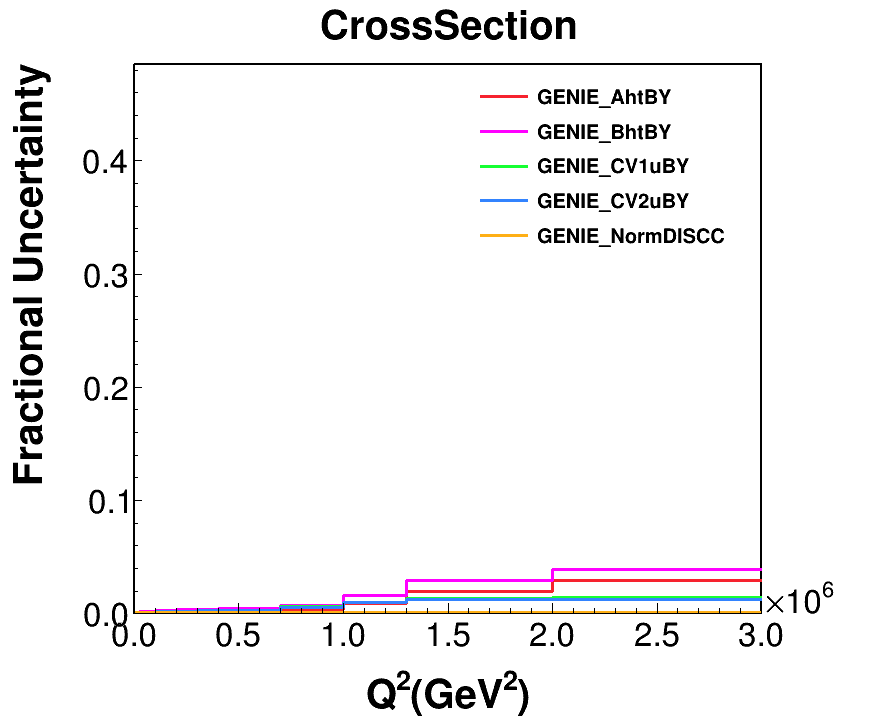
\includegraphics[scale=0.28]{Figures/AppendixB/XsecUnc1D/ErrorSummary_CrossSection_q2_Frac__1Pi_DIS-Hadronization.png}
        \caption{$\NewVar$ 1D cross section systematic error breakdown for the DIS and hadronization models. Figures by the author.}
        \label{fig:AppendixB:CrossSecModel:1DCrossSectionDISHadronization\var}
    \end{figure}  
}


%\subsection{Elastic Cross Section Models Breakdown Uncertainties}
%\label{Ap:Systematics1D:CrosSectionModels:Elastic}

\foreach \var in  {enu,mixtpi,mixthetapi_deg,pmu,ptmu,pzmu,thetamu_deg,q2,wexp}{
%\foreach \var in  {enu_true,mixtpi_true,pmu_true,ptmu_true,pzmu_true,thetamu_deg_true,q2_true,wexp_true}{
    \ifthenelse{\equal{\var}{enu}}{
      \renewcommand{\NewVar}{E_\nu}
    }{}
    \ifthenelse{\equal{\var}{mixtpi}}{
      \renewcommand{\NewVar}{T_\pi}
    }{}
    \ifthenelse{\equal{\var}{mixthetapi_deg}}{
      \renewcommand{\NewVar}{\theta_\pi}
    }{}
    \ifthenelse{\equal{\var}{pmu}}{
      \renewcommand{\NewVar}{P_\mu}
    }{}
    \ifthenelse{\equal{\var}{ptmu}}{
      \renewcommand{\NewVar}{P^T_\mu}
    }{}
    \ifthenelse{\equal{\var}{pzmu}}{
      \renewcommand{\NewVar}{P^z_\mu}
    }{}
    \ifthenelse{\equal{\var}{thetamu_deg}}{
      \renewcommand{\NewVar}{\theta_\mu}
    }{}
    \ifthenelse{\equal{\var}{q2}}{
      \renewcommand{\NewVar}{Q^2}
    }{}
    \ifthenelse{\equal{\var}{wexp}}{
      \renewcommand{\NewVar}{W_{exp}}
    }{}
    \begin{figure}[!h]
        \centering
        \includegraphics[scale=0.28]{Figures/AppendixB/XsecUnc1D/ErrorSummary_CrossSection_\var_Frac__1Pi_Elastic.png}
        \caption{$\NewVar$ 1D cross section systematic error breakdown for the Elastic interaction models. Figures by the author.}
        \label{fig:AppendixB:CrossSecModel:1DCrossSectionElastic\var}
    \end{figure}  
}
\clearpage

%\subsection{MnvTunes Cross Section Models Breakdown Uncertainties}
%\label{Ap:Systematics1D:CrosSectionModels:MnvTunes}

\foreach \var in  {enu,mixtpi,mixthetapi_deg,pmu,ptmu,pzmu,thetamu_deg,q2,wexp}{
%\foreach \var in  {enu_true,mixtpi_true,pmu_true,ptmu_true,pzmu_true,thetamu_deg_true,q2_true,wexp_true}{
    \ifthenelse{\equal{\var}{enu}}{
      \renewcommand{\NewVar}{E_\nu}
    }{}
    \ifthenelse{\equal{\var}{mixtpi}}{
      \renewcommand{\NewVar}{T_\pi}
    }{}
    \ifthenelse{\equal{\var}{mixthetapi_deg}}{
      \renewcommand{\NewVar}{\theta_\pi}
    }{}
    \ifthenelse{\equal{\var}{pmu}}{
      \renewcommand{\NewVar}{P_\mu}
    }{}
    \ifthenelse{\equal{\var}{ptmu}}{
      \renewcommand{\NewVar}{P^T_\mu}
    }{}
    \ifthenelse{\equal{\var}{pzmu}}{
      \renewcommand{\NewVar}{P^z_\mu}
    }{}
    \ifthenelse{\equal{\var}{thetamu_deg}}{
      \renewcommand{\NewVar}{\theta_\mu}
    }{}
    \ifthenelse{\equal{\var}{q2}}{
      \renewcommand{\NewVar}{Q^2}
    }{}
    \ifthenelse{\equal{\var}{wexp}}{
      \renewcommand{\NewVar}{W_{exp}}
    }{}
    \begin{figure}[!h]
        \centering
        \includegraphics[scale=0.28]{Figures/AppendixB/XsecUnc1D/ErrorSummary_CrossSection_\var_Frac__1Pi_MnvTunes.png}
        \caption{$\NewVar$ 1D cross section systematic error breakdown for the MnvTunes models. Figures by the author.}
        \label{fig:AppendixB:CrossSecModel:1DCrossSectionMnvTunes\var}
    \end{figure}  
}
\clearpage



%\subsection{No Resonant pion production Cross Section Models Breakdown Uncertainties}
%\label{Ap:Systematics1D:CrosSectionModels:NoRESpi}

\foreach \var in  {enu,mixtpi,mixthetapi_deg,pmu,ptmu,pzmu,thetamu_deg,q2,wexp}{
%\foreach \var in  {enu_true,mixtpi_true,pmu_true,ptmu_true,pzmu_true,thetamu_deg_true,q2_true,wexp_true}{
    \ifthenelse{\equal{\var}{enu}}{
      \renewcommand{\NewVar}{E_\nu}
    }{}
    \ifthenelse{\equal{\var}{mixtpi}}{
      \renewcommand{\NewVar}{T_\pi}
    }{}
    \ifthenelse{\equal{\var}{mixthetapi_deg}}{
      \renewcommand{\NewVar}{\theta_\pi}
    }{}
    \ifthenelse{\equal{\var}{pmu}}{
      \renewcommand{\NewVar}{P_\mu}
    }{}
    \ifthenelse{\equal{\var}{ptmu}}{
      \renewcommand{\NewVar}{P^T_\mu}
    }{}
    \ifthenelse{\equal{\var}{pzmu}}{
      \renewcommand{\NewVar}{P^z_\mu}
    }{}
    \ifthenelse{\equal{\var}{thetamu_deg}}{
      \renewcommand{\NewVar}{\theta_\mu}
    }{}
    \ifthenelse{\equal{\var}{q2}}{
      \renewcommand{\NewVar}{Q^2}
    }{}
    \ifthenelse{\equal{\var}{wexp}}{
      \renewcommand{\NewVar}{W_{exp}}
    }{}
    \begin{figure}[!h]
        \centering
        \includegraphics[scale=0.28]{Figures/AppendixB/XsecUnc1D/ErrorSummary_CrossSection_\var_Frac__1Pi_NonRESPi.png}
        \caption{$\NewVar$ 1D cross section systematic error breakdown for the no resonant pion models. Figures by the author.}
        \label{fig:AppendixB:CrossSecModel:1DCrossSectionNoRESpi\var}
    \end{figure}  
}




%\subsection{Resonant pion production Cross Section Models Breakdown Uncertainties}
%\label{Ap:Systematics1D:CrosSectionModels:RESpi}
\foreach \var in  {enu,mixtpi,mixthetapi_deg,pmu,ptmu,pzmu,thetamu_deg,q2,wexp}{
%\foreach \var in  {enu_true,mixtpi_true,pmu_true,ptmu_true,pzmu_true,thetamu_deg_true,q2_true,wexp_true}{
    \ifthenelse{\equal{\var}{enu}}{
      \renewcommand{\NewVar}{E_\nu}
    }{}
    \ifthenelse{\equal{\var}{mixtpi}}{
      \renewcommand{\NewVar}{T_\pi}
    }{}
    \ifthenelse{\equal{\var}{mixthetapi_deg}}{
      \renewcommand{\NewVar}{\theta_\pi}
    }{}
    \ifthenelse{\equal{\var}{pmu}}{
      \renewcommand{\NewVar}{P_\mu}
    }{}
    \ifthenelse{\equal{\var}{ptmu}}{
      \renewcommand{\NewVar}{P^T_\mu}
    }{}
    \ifthenelse{\equal{\var}{pzmu}}{
      \renewcommand{\NewVar}{P^z_\mu}
    }{}
    \ifthenelse{\equal{\var}{thetamu_deg}}{
      \renewcommand{\NewVar}{\theta_\mu}
    }{}
    \ifthenelse{\equal{\var}{q2}}{
      \renewcommand{\NewVar}{Q^2}
    }{}
    \ifthenelse{\equal{\var}{wexp}}{
      \renewcommand{\NewVar}{W_{exp}}
    }{}
    \begin{figure}[!h]
        \centering
        \includegraphics[scale=0.28]{Figures/AppendixB/XsecUnc1D/ErrorSummary_CrossSection_\var_Frac__1Pi_RESPi.png}
        \caption{$\NewVar$ 1D cross section systematic error breakdown for the Resonant pion production models. Figures by the author.}
        \label{fig:AppendixB:CrossSecModel:1DCrossSectionRESpi\var}
    \end{figure}  
}

\pagebreak

\section{Genie FSI Uncertainties}
\label{Ap:Systematics1D:FSI}

\foreach \var in  {enu,mixtpi,mixthetapi_deg,pmu,ptmu,pzmu,thetamu_deg,q2,wexp}{
%\foreach \var in  {enu_true,mixtpi_true,pmu_true,ptmu_true,pzmu_true,thetamu_deg_true,q2_true,wexp_true}{
    \ifthenelse{\equal{\var}{enu}}{
      \renewcommand{\NewVar}{E_\nu}
    }{}
    \ifthenelse{\equal{\var}{mixtpi}}{
      \renewcommand{\NewVar}{T_\pi}
    }{}
    \ifthenelse{\equal{\var}{mixthetapi_deg}}{
      \renewcommand{\NewVar}{\theta_\pi}
    }{}
    \ifthenelse{\equal{\var}{pmu}}{
      \renewcommand{\NewVar}{P_\mu}
    }{}
    \ifthenelse{\equal{\var}{ptmu}}{
      \renewcommand{\NewVar}{P^T_\mu}
    }{}
    \ifthenelse{\equal{\var}{pzmu}}{
      \renewcommand{\NewVar}{P^z_\mu}
    }{}
    \ifthenelse{\equal{\var}{thetamu_deg}}{
      \renewcommand{\NewVar}{\theta_\mu}
    }{}
    \ifthenelse{\equal{\var}{q2}}{
      \renewcommand{\NewVar}{Q^2}
    }{}
    \ifthenelse{\equal{\var}{wexp}}{
      \renewcommand{\NewVar}{W_{exp}}
    }{}
    \begin{figure}[!h]
        \centering
        \includegraphics[scale=0.28]{Figures/AppendixB/XsecUnc1D/ErrorSummary_CrossSection_\var_Frac__1Pi_GENIE_FSI.png}
        \caption{$\NewVar$ 1D cross section systematic error breakdown for the FSI models. Figures by the author.}
        \label{fig:AppendixB:CrossSecModel:1DFSImodel\var}
    \end{figure}  
}
\clearpage




%\subsection{CCQE Cross Section Models Breakdown Uncertainties}
%\label{Ap:Systematics1D:CrosSectionModels:CCQE}



\pagebreak


\section{Muon Uncertainties}
\label{Ap:Systematics1D:Muon}

\foreach \var in  {enu,mixtpi,mixthetapi_deg,pmu,ptmu,pzmu,thetamu_deg,q2,wexp}{
%\foreach \var in  {enu_true,mixtpi_true,pmu_true,ptmu_true,pzmu_true,thetamu_deg_true,q2_true,wexp_true}{
    \ifthenelse{\equal{\var}{enu}}{
      \renewcommand{\NewVar}{E_\nu}
    }{}
    \ifthenelse{\equal{\var}{mixtpi}}{
      \renewcommand{\NewVar}{T_\pi}
    }{}
    \ifthenelse{\equal{\var}{mixthetapi_deg}}{
      \renewcommand{\NewVar}{\theta_\pi}
    }{}
    \ifthenelse{\equal{\var}{pmu}}{
      \renewcommand{\NewVar}{P_\mu}
    }{}
    \ifthenelse{\equal{\var}{ptmu}}{
      \renewcommand{\NewVar}{P^T_\mu}
    }{}
    \ifthenelse{\equal{\var}{pzmu}}{
      \renewcommand{\NewVar}{P^z_\mu}
    }{}
    \ifthenelse{\equal{\var}{thetamu_deg}}{
      \renewcommand{\NewVar}{\theta_\mu}
    }{}
    \ifthenelse{\equal{\var}{q2}}{
      \renewcommand{\NewVar}{Q^2}
    }{}
    \ifthenelse{\equal{\var}{wexp}}{
      \renewcommand{\NewVar}{W_{exp}}
    }{}
    \begin{figure}[!h]
        \centering
        \includegraphics[scale=0.28]{Figures/AppendixB/XsecUnc1D/ErrorSummary_CrossSection_\var_Frac__1Pi_Muon.png}
        \caption{$\NewVar$ 1D cross section systematic error breakdown for the associated muon kinematics measurements. Figures by the author. }
        \label{fig:AppendixB:CrossSecModel:1DMuon\var}
    \end{figure}  
}
\clearpage



\section{Pion Reconstruction Uncertainties}
\label{Ap:Systematics1D:PionReconstruction}

\foreach \var in  {enu,mixtpi,mixthetapi_deg,pmu,ptmu,pzmu,thetamu_deg,q2,wexp}{
%\foreach \var in  {enu_true,mixtpi_true,pmu_true,ptmu_true,pzmu_true,thetamu_deg_true,q2_true,wexp_true}{
    \ifthenelse{\equal{\var}{enu}}{
      \renewcommand{\NewVar}{E_\nu}
    }{}
    \ifthenelse{\equal{\var}{mixtpi}}{
      \renewcommand{\NewVar}{T_\pi}
    }{}
    \ifthenelse{\equal{\var}{mixthetapi_deg}}{
      \renewcommand{\NewVar}{\theta_\pi}
    }{}
    \ifthenelse{\equal{\var}{pmu}}{
      \renewcommand{\NewVar}{P_\mu}
    }{}
    \ifthenelse{\equal{\var}{ptmu}}{
      \renewcommand{\NewVar}{P^T_\mu}
    }{}
    \ifthenelse{\equal{\var}{pzmu}}{
      \renewcommand{\NewVar}{P^z_\mu}
    }{}
    \ifthenelse{\equal{\var}{thetamu_deg}}{
      \renewcommand{\NewVar}{\theta_\mu}
    }{}
    \ifthenelse{\equal{\var}{q2}}{
      \renewcommand{\NewVar}{Q^2}
    }{}
    \ifthenelse{\equal{\var}{wexp}}{
      \renewcommand{\NewVar}{W_{exp}}
    }{}
    \begin{figure}[!h]
        \centering
        \includegraphics[scale=0.28]{Figures/AppendixB/XsecUnc1D/ErrorSummary_CrossSection_\var_Frac__1Pi_Pion_Reconstruction.png}
        \caption{$\NewVar$ 1D cross section systematic error breakdown for the associated pion reconstruction. Figures by the author. }
        \label{fig:AppendixB:CrossSecModel:1DPionReconstruction\var}
    \end{figure}  
}
\clearpage


\section{Flux Uncertainties}
\label{Ap:Systematics1D:Flux}

\foreach \var in  {enu,mixtpi,mixthetapi_deg,pmu,ptmu,pzmu,thetamu_deg,q2,wexp}{
%\foreach \var in  {enu_true,mixtpi_true,pmu_true,ptmu_true,pzmu_true,thetamu_deg_true,q2_true,wexp_true}{
    \ifthenelse{\equal{\var}{enu}}{
      \renewcommand{\NewVar}{E_\nu}
    }{}
    \ifthenelse{\equal{\var}{mixtpi}}{
      \renewcommand{\NewVar}{T_\pi}
    }{}
    \ifthenelse{\equal{\var}{mixthetapi_deg}}{
      \renewcommand{\NewVar}{\theta_\pi}
    }{}
    \ifthenelse{\equal{\var}{pmu}}{
      \renewcommand{\NewVar}{P_\mu}
    }{}
    \ifthenelse{\equal{\var}{ptmu}}{
      \renewcommand{\NewVar}{P^T_\mu}
    }{}
    \ifthenelse{\equal{\var}{pzmu}}{
      \renewcommand{\NewVar}{P^z_\mu}
    }{}
    \ifthenelse{\equal{\var}{thetamu_deg}}{
      \renewcommand{\NewVar}{\theta_\mu}
    }{}
    \ifthenelse{\equal{\var}{q2}}{
      \renewcommand{\NewVar}{Q^2}
    }{}
    \ifthenelse{\equal{\var}{wexp}}{
      \renewcommand{\NewVar}{W_{exp}}
    }{}
    \begin{figure}[!h]
        \centering
        \includegraphics[scale=0.28]{Figures/AppendixB/XsecUnc1D/ErrorSummary_CrossSection_\var_Frac__1Pi_Flux.png}
        \caption{$\NewVar$ 1D cross section systematic error breakdown for the associated to the neutrino flux. Figures by the author.}
        \label{fig:AppendixB:CrossSecModel:1DFlux\var}
    \end{figure}  
}
\clearpage

\section{Others Uncertainties}
\label{Ap:Systematics1D:Others}

\foreach \var in  {enu,mixtpi,mixthetapi_deg,pmu,ptmu,pzmu,thetamu_deg,q2,wexp}{
%\foreach \var in  {enu_true,mixtpi_true,pmu_true,ptmu_true,pzmu_true,thetamu_deg_true,q2_true,wexp_true}{
    \ifthenelse{\equal{\var}{enu}}{
      \renewcommand{\NewVar}{E_\nu}
    }{}
    \ifthenelse{\equal{\var}{mixtpi}}{
      \renewcommand{\NewVar}{T_\pi}
    }{}
    \ifthenelse{\equal{\var}{mixthetapi_deg}}{
      \renewcommand{\NewVar}{\theta_\pi}
    }{}
    \ifthenelse{\equal{\var}{pmu}}{
      \renewcommand{\NewVar}{P_\mu}
    }{}
    \ifthenelse{\equal{\var}{ptmu}}{
      \renewcommand{\NewVar}{P^T_\mu}
    }{}
    \ifthenelse{\equal{\var}{pzmu}}{
      \renewcommand{\NewVar}{P^z_\mu}
    }{}
    \ifthenelse{\equal{\var}{thetamu_deg}}{
      \renewcommand{\NewVar}{\theta_\mu}
    }{}
    \ifthenelse{\equal{\var}{q2}}{
      \renewcommand{\NewVar}{Q^2}
    }{}
    \ifthenelse{\equal{\var}{wexp}}{
      \renewcommand{\NewVar}{W_{exp}}
    }{}
    \begin{figure}[!h]
        \centering
        \includegraphics[scale=0.28]{Figures/AppendixB/XsecUnc1D/ErrorSummary_CrossSection_\var_Frac__1Pi_Others.png}
        \caption{$\NewVar$ 1D cross section systematic error breakdown. Figures by the author. }
        \label{fig:AppendixB:CrossSecModel:1DOther\var}
    \end{figure}  
}
\clearpage


